\documentclass[../main/main.tex]{subfiles}

\newdate{date}{24}{03}{2020}

\begin{document}

\marginpar{ \textbf{Lecture 5.} \\  \displaydate{date}. \\ Compiled:  \today.}

In summary, we have derived the second quantization form of the interaction potential term as a function of creation and destruction operators.

Now, in order to proceed, it is convenient to split the sum \( \sum_{\va{k},\va{p},\va{q}}^{}   \) into two parts: a part corresponding to \( \va{q}=0 \) and the rest containing terms with \( \va{q}\neq0 \).

Firstly, let us consider the \( \va{q}=0 \) term: \marginpar{\( \va{q=0} \) term}
\begin{equation*}
  \hat{V} (\va{q}=0) = \frac{e^2}{2V} \frac{4 \pi }{\mu ^2} \sum_{\substack{\va{k} \va{p}\\ \lambda \mu  } }^{}  a_{\va{k} \lambda } ^\dag \mathcolorbox{green!20}{a_{\va{p} \mu } ^\dag a_{\va{p} \mu } a_{\va{k} \lambda }}
\end{equation*}
By recalling the commutation rules:
\begin{equation*}
[\hat{n}_{\va{p} \mu }, a_{\va{k} \lambda } ] =
[a_{\va{p} \mu } ^\dag a_{\va{p} \mu }, a_{\va{k} \lambda } ]
= \mathcolorbox{green!20}{a_{\va{p} \mu }^\dag a_{\va{p} \mu } a_{\va{k}\lambda }} - a_{\va{k} \lambda } a_{\va{p} \mu }^\dag a_{\va{p} \mu }
= - \delta _{\va{k} \va{p}} \delta _{\mu \lambda } a_{\va{k} \lambda }
\end{equation*}
where the green term is corresponding to the green term in the \( \hat{V} (\va{q}=0)  \) contribution; hence, we can rewrite:
\begin{equation*}
 a_{\va{p} \mu } ^\dag a_{\va{p} \mu } a_{\va{k} \lambda }
 = a_{\va{k} \lambda } a_{\va{p} \mu } ^\dag a_{\va{p} \mu }
 - \delta _{\va{k} \va{p}} \delta _{\mu \lambda } a_{\va{k} \lambda }
 = a_{\va{k}\lambda } \qty(  a_{\va{p} \mu } ^\dag a_{\va{p} \mu } - \delta _{\va{k} \va{p}} \delta _{\mu \lambda } )
\end{equation*}
Eventually, we can rewrite:
\begin{equation*}
\begin{split}
  \hat{V} \qty(\va{q} = 0) &= \frac{e^2}{2V}  \frac{4 \pi }{\mu ^2}
  \sum_{\substack{\va{k} \va{p}\\ \lambda  \mu  } }^{}
  \underbrace{a_{\va{k} \lambda } ^\dag a_{\va{k} \lambda }}_{\hat{n}_{\va{k}\lambda } }
  \qty( \underbrace{a_{\va{p} \mu }^\dag a_{\va{p} \mu } }_{\hat{n}_{\va{p} \mu } } - \delta _{\va{k} \va{p}} \delta _{\mu \lambda }  )   \\
  & \overset{(a)}{=}  \frac{e^2}{2V}  \frac{4 \pi }{\mu ^2} \underbrace{ \qty(\sum_{\va{k}\lambda }^{} \hat{n}_{\va{k} \lambda }   )  }_{\hat{N} }
  \underbrace{\qty(\sum_{\va{p} \mu }^{} \hat{n}_{\va{p} \mu }   ) }_{\hat{N} }
  -  \frac{e^2}{2V}  \frac{4 \pi }{\mu ^2} \underbrace{ \qty( \sum_{\va{k} \lambda }^{} \hat{n}_{\va{k} \lambda }    )  }_{\hat{N} } \\
  & \overset{(b)}{=}  \frac{e^2}{2V}  \frac{4 \pi }{\mu ^2} \qty(\hat{N}^2 - \hat{N}  )
  \overset{(c)}{=} \frac{e^2}{2V}  \frac{4 \pi }{\mu ^2} \qty(N^2 - N)
\end{split}
\end{equation*}
where in \( (a) \) we have separated the two sum over   \( \va{k} \) and \( \va{p} \) and in \( (b) \) we have noted that by definition the sum of the number operator over all the wave vectors and spins gives the operator \( \hat{N}  \).
Actually, in \( (c) \)  we treated it as a \( c \)-number (\( \hat{N} \rightarrow N  \)) because we are working with a constant number of particles and, in particular, this operator commutes with the total hamiltonian: \( [\hat{H},\hat{N}  ] = 0 \).




We should also consider the thermodynamic limit: first of all we let \( V \rightarrow \infty  \) and the we take the limit \( \mu \rightarrow 0 \). Let us remind that the correct order is important, indeed the energy is an extensive quantity and if we consider the energy per particle we obtain:
\begin{equation*}
  \frac{e^2}{2V}  \frac{4 \pi }{\mu ^2} \qty(N^2-N) \frac{1}{N}
  = \frac{e^2}{2}  \frac{4 \pi }{\mu ^2} \qty(\frac{N}{V}) - \cancel{\frac{e^2}{2}  \frac{4 \pi }{\mu ^2} \frac{1}{V}}
\end{equation*}
where the second term vanishes in the thermodynamic limit, while we take \( \mu  \) finite in a way such that the above equation is describes a well defined quantity.

In practice, our \( \va{q}=0 \) contribution reduces to:
\begin{equation*}
  \hat{V} (\va{q}=0) \simeq \frac{e^2}{2} \frac{4 \pi }{\mu ^2} \frac{N^2}{V}>0
\end{equation*}
that is a repulsion term between electrons (to be more precise, since \( \va{q}=0 \)  it is a repulsion between \emph{uniform} portion of electrons).

If we now sum this term to the others two terms \( H_b \) and \( H_{el-b} \), we get that the results is equal to zero:
\begin{equation*}
  H_b + H_{el-b} + \hat{V}  (\va{q}=0) = 0
\end{equation*}
In other words, \( \hat{V}  (\va{q}=0) \)  completely cancels the remaining \marginpar{Cancel divergences}  divergences that we had before. This is what we expected, since the system is neutral and that if we come back to the original expression of \( \hat{V}  \) (without the splitting of the sum), what remains is just the expression were we restrict to the sum over \( \va{q} \) different from zero:
\begin{equation*}
  \hat{V} =  \frac{e^2}{2V} \sum_{\substack{\va{k}\va{p}\va{q} \\ \lambda \mu } }^{'} \frac{4 \pi }{q^2+\mu ^2} a_{\va{k}+ \va{q}, \lambda } ^\dag
  a_{\va{p}-\va{q}, \mu } ^\dag a_{\va{p}\mu }a_{\va{k} \lambda }
\end{equation*}
where we have written the sum as \( \sum_{}^{'}   \) just to remember that we must take into account only the \( \va{q} \neq 0 \) contribution.
Of course, now there are no longer convergence problems and we can safely take the limit \( \mu \rightarrow 0 \), in such a way to recover the genuine Coulomb interaction and we obtain:
\begin{equation*}
  \hat{V} = \frac{e^2}{2V}\sum_{\substack{\va{k}\va{p}\va{q} \\ \lambda \mu } }^{'}
  \frac{4 \pi }{q^2} a_{\va{k}+ \va{q}, \lambda } ^\dag
  a_{\va{p}-\va{q}, \mu } ^\dag a_{\va{p}\mu }a_{\va{k} \lambda }
\end{equation*}
Hence, the \( \va{q}\neq 0 \) terms describe the electron-electron interactions that survive after the divergences cancellation. 


\subsubsection{Total Hamiltonian}
Finally, the complete Hamiltonian of the degenerate electron gas is the following: \marginpar{Hamiltonian of the system in second quantization}
\begin{equation}
  \hat{H} = \sum_{\va{k} \lambda }^{} \frac{\hbar ^2 k^2}{2m} a_{\va{k}\lambda }^\dag a_{\va{k}\lambda } + \frac{e^2}{2V} \sum_{\substack{\va{k}\va{p}\va{q} \\ \lambda \mu  } }^{'} \frac{4 \pi }{q^2} a_{\va{k}+\va{q}, \lambda } ^\dag  a_{\va{p}-\va{q}, \mu } ^\dag a_{\va{p}\mu }a_{\va{k} \lambda }
\end{equation}
where the first term corresponds to the kinetic energy term and the second one to the  potential energy term  where we have to remember that in the sum we should consider only \( q \neq 0 \) terms.
Hence, up to now we have not done nothing new: we have only rewritten the Hamiltonian in the second quantization form both for the kinetic and potential terms.

In order to proceed we need to do a further observation: this Jellium model is drastic approximation of a real metal and of course we have missed the information of some characteristic properties of a real metal such as the lattice parameter, the interatomic distance and so on and so forth. Essentially, our model is just characterized by two quantities, i.e. the two characteristic lengths of the system: \marginpar{Characteristic lengths: \( r_0 \) and \( a_0 \)}
\begin{itemize}
\item the \textbf{interparticle distance} (electron-electron), which is called \( r_0 \). Imagine we assign a small spherical volume \( V_0 \) to each electron, the total volume can be written as (it is not possible to fill the whole space, but we have in mind only the order of magnitude of \( r_0 \)):
\begin{equation*}
  V_0 = \frac{4 \pi }{3} r_0^3 \quad \rightarrow V = N V_0 = \frac{4 \pi }{3} r_0^3 N
\end{equation*}
where \( N \) is the total number of particles. Clearly, using this expression one can immediately write the expression of the \( r_0 \) parameter:
\begin{equation*}
  V_0 = \frac{V}{N} = \frac{1}{n} \quad \rightarrow r_0 = \qty(\frac{3}{4 \pi n})^{1/3}
\end{equation*}
This distance is important because because even though we have no special property in our Jellium model, in order to mimic real metal behavior, what we can do is to define the density and thus we can define the interparticle distance \( r_0 \).

\item the \textbf{Bohr radius} \( a_0 \) is a relevant distance because the kind of interaction between electron-electron and backgorund-electrons is a Coulomb one.
In particular, the Bohr radius corresponds to the radius of the Hydrogen atom in its ground state in which there is a Coulomb interaction between the electron and the proton of the atom. Hence, the Bohr radius is another characteristic length which is related to the kind of interaction which acts in our system.
\end{itemize}
The dimensionless ratio between these two lengths results:
\begin{equation*}
  r_s \equiv \frac{r_0}{a_0}
\end{equation*}
which corresponds to the interparticle spacing in terms of the Bohr radius and characterizes the density of the system.
\begin{remark}
\( r_s \)  is a common parameter to characterize the Jellium model, for instance by taking into account the density of real metals, the value of \( r_s \) is between 2 and 6.
\end{remark}
Now, since we have introduce those two parameters \( r_0,a_0 \) and this dimensionless quantity \( r_s \), we can also define other dimensionless quantities as:
\begin{equation*}
  \bar{V} \equiv \frac{V}{r_0^3}, \quad \bar{\va{k}} \equiv r_0 \va{k}, \quad  \bar{\va{p}} \equiv r_0 \va{p}, \quad \bar{\va{q}} \equiv r_0 \va{q}
\end{equation*}
For example:
\begin{itemize}
\item for the \emph{kinetic term}:
\begin{equation*}
  a_0 = \frac{\hbar ^2}{m e^2} \quad \rightarrow \frac{\hbar ^2}{m} = a_0 e^2
\end{equation*}
\item for the \emph{potential term}:
\begin{equation*}
  \frac{e^2}{V} \frac{1}{q^2} = \frac{e^2}{\bar{V}r_0^3 }\frac{r_0^2}{\bar{q}^2 }
  = \frac{e^2}{\bar{V}\bar{q}^2  }\frac{1}{r_s a_0}
  = \qty(\frac{e^2}{2 a_0}) \frac{2}{r_s^2} \frac{r_s}{\bar{V}\bar{q}^2  }
\end{equation*}
\end{itemize}
Now, by taking into account this change in term of dimensionless variable, we can rewrite the Hamiltonian in second quantization in this way:
\begin{equation}
  \hat{H} = \frac{e^2}{a_0 r_s^2} \qty(\underbrace{\sum_{\va{k} \lambda }^{} \frac{1}{2} \bar{k}^2 a_{\bar{\va{k}} \lambda  } ^\dag  a_{\bar{\va{k}} \lambda  } }_{\hat{H}_0 }
  +  \underbrace{ \frac{ \mathcolorbox{green!20}{r_s}}{2 \bar{V} } \sum_{\bar{\va{k}}\bar{\va{p}} \bar{\va{q}}  }^{'} \sum_{\lambda  \mu }^{} \frac{4 \pi }{\bar{q}^2 } a_{\bar{\va{k}}+\bar{\va{q}}, \lambda   } ^\dag a_{\bar{\va{p}}-\bar{\va{q}}, \mu   } ^\dag  a_{\bar{\va{p}} \mu } a_{\bar{\va{k}}, \lambda  }   }_{\hat{H}_1 }   ) = \frac{e^2}{a_0 r_s^2} \qty( \hat{H}_0 + \hat{H}_1 )
\end{equation}
where we have inside the parenthesis the same quantities as before, with the only difference that we have replaced the quantities with their correspondent dimensionless one and we have the \( r_s \) parameter in the potential energy term.
Note that the term in front of the parenthesis can be written also as:
\begin{equation*}
  \frac{e^2}{a_0 r_s^2} = \qty(\frac{e^2}{2 a_0}) \frac{2}{r_s^2} = \qty(1 \text{ Ryd}) \vdot \frac{2}{r_s^2}
\end{equation*}
where \( 1 \text{ Ryd} = \SI{13.6}{\eV}  \), the neutral unit for the energy (the ground state energy of the hydrogen atom).

\subsubsection{Perturbative approach}

The most important result is that we can rewrite schematically the Hamiltonian as the sum of \( \hat{H}_0  \)  and \( \hat{H}_1  \) contributions, where the first term is just the kinetic term and the second term is  the potential interaction term, which is multiplied by the \( r_s \) parameter. The latter, is the goal of this derivation because it implies that as \( r_s \rightarrow 0 \), the potential energy becomes a small perturbation. It is a contro-intuitive result, because it means that in high-density limit the electron-electron interaction becomes smaller with respect to the kinetic dominant contribution.  \marginpar{Perturbative approach}
In practice, in the so high-density limit, we expect that a perturbative approach, starting from a non interacting system, is possible even though the Coulomb potential is neither weak nor short-range.

One could expect that just considering few terms in the perturbative approach could give a good result. Unfortunately, while one can easily evaluate the \emph{leading term} in the interaction energy (i.e. the \( 1^{st} \) order perturbation theory), several problems appear considering higher-oders (for instance the \( 2^{nd} \) order term diverges logarithmically!).
The total energy can be rewritten as: \marginpar{Total energy in perturbative form}
\begin{equation}
  E = \frac{N e^2}{a_0 r_s^2} \qty(\mathcolorbox{green!20}{a} + \mathcolorbox{yellow!40}{b r_s} + \mathcolorbox{red!30}{c r_s^2 \ln{r_s}} + \dots )
  \label{eq:5_1}
\end{equation}
where the green term represents a constant, the yellow term the \( 1^{st} \) order approximation term and the red term the \( 2^{nd} \) order one, where we can see the exponential divergence in the limit \( r_s \rightarrow 0 \).

To summarize, we have shown that the potential energy of our Jellium model becomes a small perturbation as the density of the system becomes higher, i.e. in the limit \( r_s \rightarrow 0  \). We have also anticipated that unfortunately it is not trivial to perform a perturbative approach just considering few orders in the perturbative expansion, because yet in the second term one find problems. More specifically, we will see it will be necessary to consider an infinite number of terms in order to have convergence of the result.

Now we evaluate the \( a \) and \( b \) parameters, namely the first two terms in the perturbative series (the zero order correction and the first order one).

\subsubsection{Unperturbed hamiltonian \(\pmb{\hat{H}_0}\)}
Let us start considering
\begin{equation*}
  \hat{H}_0 = \sum_{\va{k} \lambda }^{} \frac{\hbar ^2 k^2}{2m} a_{\va{k} \lambda } ^\dag a_{\va{k}\lambda } = \sum_{\va{k}\lambda }^{} \frac{\hbar ^2 k^2}{2m} \hat{n}_{\va{k} \lambda }
\end{equation*}
that is the unperturbed Hamiltonian representing a \emph{non-interacting} Fermi system (while \(\hat{H}_1\) is the small perturbation). In practice, this is the zero order term in the perturbative approach, which as expected is easy to treat because in this term we describe only non-interacting particles.
Now, the problem is what is our system when the particle are non interacting, the idea is simple: the system obeys the Pauli exclusion principle. Indeed, due to the Pauli exclusion principle each momentum (or wave vector) eigenstate (each single-particle state) can be occupied by only two electrons: one with spin-up and one with spin-down.
Essentially, the \emph{ground state} of the non-interacting degenerate electron gas is the so called \textbf{Fermi sphere} \marginpar{Fermi sphere}, a sphere in the momentum space (or in the reciprocal space), and the ground state is represented as \( \ket{F}  \).
In particular, inside the sphere we have all the occupied states, while outside the empty ones. The Fermi sphere is thus obtained by filling it with single-particle states up to a \emph{maximum value} (depending on the total number of particles), that is called the \textbf{Fermi momentum}: \marginpar{
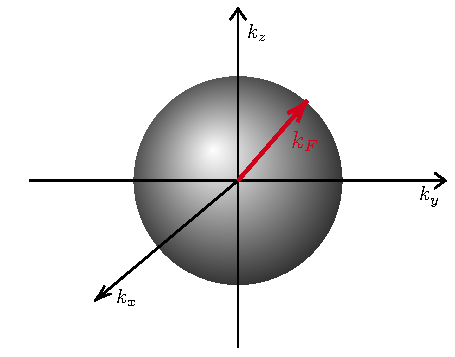
\includegraphics[width=\marginparwidth]{../lessons/5_image/1.pdf}
\captionof{figure}{\label{fig:} Fermi sphere.}
}
\begin{equation*}
  p_F = \hbar k_F
\end{equation*}
that is the product of the \textbf{Fermi wave vector} per \( \hbar  \).
Clearly, the occupied states are denoted by states where:
\begin{equation*}
  \abs{\va{k}} \le \abs{\va{k}_F}
\end{equation*}
We have to respect also the boundary conditions:
\begin{equation*}
  \va{k} = \frac{2 \pi }{L}\va{n}
\end{equation*}
Thus, the spacing between the \( \va{k} \) value is:
\begin{equation*}
  \Delta k_ \alpha = \frac{2 \pi }{L} \quad \alpha =x,y,z \quad \rightarrow   \abs{\Delta \va{k}}  = \frac{(2 \pi )^3}{L^3}
\end{equation*}
it corresponds to a small cube assigned in the reciprocal space to every state \( \abs{\Delta \va{k}}  \).

Now, lets try to make the sum over all these states::
\begin{equation*}
  \sum_{\abs{\va{k}}\le k_F }^{} 1 = \frac{N}{2}
\end{equation*}
this must be equal to the total number of particle divided by a factor 2, because ,due to spin degeneracy, every single state characterized by a given value of the \( \va{k} \)  wave vector can be occupied by up to two electrons (spin-up and spin-down).
Now, it is convenient to work in the thermodynamic limit \( L \rightarrow \infty  \) to replace the discrete sum with an integral over \( \va{k} \) (it is convenient because in general we know better how to solve and integral than the corresponding sum). In practice we can transform the sum into an integral as follow:
\begin{equation}
  \sum_{\va{k }}^{} = \sum_{\va{k}}^{} \frac{\abs{\Delta \va{k}} }{\abs{\Delta \va{k}} } = \frac{1}{\abs{\Delta \va{k}} }  \sum_{\va{k}}^{}  \abs{\Delta \va{k}}
  \overset{L \rightarrow \infty }{\rightarrow  } \frac{V}{(2 \pi )^3} \int_{}^{} \dd[]{\va{k}}
  \label{eq:5_2}
\end{equation}
In practice, in our specific case:
\begin{equation*}
  \sum_{\abs{\va{k}} \le k_F }^{}   \overset{L \rightarrow \infty }{\rightarrow  }
  \frac{V}{(2 \pi )^3} \int_{\abs{\va{k}} \le k_F}^{} \dd[]{\va{k}}
  = \frac{V}{(2 \pi )^3} \mathcolorbox{green!20}{\frac{4 \pi }{3} k_F^3} = \frac{N}{2}
\end{equation*}
where the green term is the volume of the Fermi sphere.
With such a relation we can directly relate the Fermi wave vector \( k_F \) to the particle density (\( N/V\)):
\begin{equation*}
  k_F = \qty(3 \pi ^2 n)^{1/3} \sim n^{1/3}
\end{equation*}

Let us evaluate the 0-order term in the perturbative approach, i.e. the energy for the non-interacting system:
\begin{equation*}
  E_0 = \bra{F} \hat{H}_0 \ket{F} = \sum_{\va{k} \lambda }^{} \frac{\hbar ^2 k^2}{2m }     \bra{F} \hat{n}_{\va{k}\lambda } \ket{F}
\end{equation*}
which is just the kinetic energy contribution and it is estimated by taking the matrix element between the unperturbed ground state.
Then, we have written it in second quantization and since by its definition the effect of the number operator multiplied to a state just gives the occupation of the state itself and  since  \( \hat{n}_{\va{k} \lambda }  \) refers to the wave vector \( \va{k} \) with spin \( \lambda  \), this gives:
\begin{equation*}
  \begin{cases}
   \hat{n}_{\va{k} \lambda } \ket{F} = \ket{F} & \text{if } \abs{\va{k}} \le k_F  \\
  \hat{n}_{\va{k} \lambda } \ket{F} = 0  & \text{if } \abs{\va{k}} > k_F
  \end{cases}
\end{equation*}
with the normalization condition on the ground state \(  \braket{F}{F}=1   \).

Clearly, we can easily evaluate the matrix element in \( E_0 \):
\begin{equation*}
  E_0 = 2 \sum_{\abs{\va{k}} \le k_F }^{}  \frac{\hbar ^2 k^2}{2m}
\end{equation*}
where the 2 factor derives from the sum over the spins \( \lambda  \) (for each state it can be occupied by two electrons with spin-up and spin-down).
Now, we go to the thermodynamic limit and since the integral depends only on the modulus of \( \va{k} \) we can immediately evaluate the spherical integral in the second step. Hence, the total energy the ground state of the non-interacting system results:
\begin{equation*}
\begin{split}
  E_0 & \overset{L \rightarrow \infty }{\rightarrow } \frac{V}{(2 \pi )^3}
  2  \int_{\abs{\va{k}} \le k_F}^{} \dd[]{\va{k}} \frac{\hbar ^2 k^2}{2m}
  =   \frac{V}{(2 \pi )^3} \cancel{2} \frac{4 \pi \hbar ^2}{\cancel{2}m }
  \int_{0}^{k_F} \dd[]{k} k^4
   \\
   & = \frac{V \hbar ^2}{2 \pi ^2 m} \frac{k_F^5}{5}
   \overset{k_F^3=3 \pi ^2 \frac{N}{V}}{=} \frac{3}{5} \underbrace{\qty(\frac{\hbar ^2 k_F^2}{2m}) }_{\varepsilon _F} N = \frac{3}{5} \varepsilon _F N
\end{split}
\end{equation*}
where we have defined the \textbf{Fermi energy} as \( \varepsilon _F \).
Let us notice that: \marginpar{Fermi energy}
\begin{equation*}
  \frac{E_0}{N} = \frac{3}{5} \varepsilon _F > 0
\end{equation*}
so if we compute the energy per particle, the result is positive (the Fermi energy is of order of few \( \SI{}{\eV}  \)) and in particular, even at zero temperature (remind that we implictly assume that we are working at \( T=0 \)) the total energy of the system is not zero but finite and positive.
As said, this is a consequence of the Pauli exclusion principle, because when we try to occupy the states in the Fermi sphere, with particle different from bosons, we cannot put all the electrons in the lowest energy state but we should occupy also states at finite energy.

Now, let us manipulate a little the expression of  \( k_F^3 \):
\begin{equation*}
  k_F^3 = 3 \pi ^2 n = \frac{3 \pi ^2}{V_0} =
  \frac{3 \pi ^2 3}{4 \pi r_0^3} = \frac{9 \pi }{4 r_0^3} =
  \frac{9 \pi }{4 r_s^3 a_0^3}
\end{equation*}
where \(V_0\) is the small volume associated to each electron.
Hence, the Fermi energy can be expressed as:
\begin{equation*}
  \varepsilon _F = \frac{\hbar ^2 k_F^2}{2m} = \frac{\hbar ^2}{2m} \qty(\frac{9 \pi }{4})^{2/3} \frac{1}{r_s^2 a_0^2}
  = \qty(\frac{e^2}{2 a_0})  \mathcolorbox{yellow!40}{\underbrace{\qty(\frac{1}{e^2} \frac{\hbar ^2}{m a_0})}_{=1}  }
  \qty(\frac{9 \pi }{4})^{2/3 }    \frac{1}{r_s^2}
  = \qty(\frac{e^2}{2 a_0})    \qty(\frac{9 \pi }{4})^{2/3 }    \frac{1}{r_s^2}
\end{equation*}
where the yellow term is equal to 1 because is just the definition of the Bohr radius. Thus we can write:
\begin{equation*}
  E_0 = \frac{3}{5} \qty(\frac{e^2}{2 a_0})    \qty(\frac{9 \pi }{4})^{2/3 }    \frac{1}{r_s^2} N
  = 2.21 \underbrace{ \qty(\frac{e^2}{2 a_0})}_{= 1 \text{Ryd}}  \frac{1}{r_s^2} N
  = \frac{2.21}{r_s^2} N \, \text{Ryd}
\end{equation*}
where we have estimated the numerical value using the definition of Rydberg, namely the ground state energy of the Hydrogen atom.
The energy is an extensive quantity and as expected it is proportional to the number of particle:
\begin{equation*}
  E_0 \sim N
\end{equation*}
Moreover, the energy \( E_0 \) goes as the inverse of the square of \( r_s \):
\begin{equation*}
  E_0 \sim \frac{1}{r_s^2}
\end{equation*}
this is the zero order perturbative expansion of \( E \) (see Eq.\eqref{eq:5_1}).
It means that \( E_0 \) is larger if the density is high, so if \( r_s \rightarrow 0 \) (i.e. if the volume per particle is small).
From a physical point of view this means that the kinetic energy contribution is larger for a more concentrated system.
Clearly, we can also understand this behavior also on the basis of the \emph{uncertainty principle}: if we force particles to be very close to each other (because of the high density), we constraint their position to be very close but the uncertainty principle has as a consequence that there is a large uncertainty on the momentum. Hence, the kinetic energy which is proportional to the square of momentum, is large.

To summarize, we have evaluated the ground state energy for non-interacting system and since non-interacting behavior its evaluation was relatively easy.
Then we have seen that this term has a larger value, if the density of the system system is high.
The next step is try to evaluate the first order correction, in particular we should try to compute the \( b \) parameter.





\end{document}
